\PassOptionsToPackage{svgnames}{xcolor}
\documentclass[12pt]{article}



\usepackage[margin=1in]{geometry}  
\usepackage{graphicx}             
\usepackage{amsmath}              
\usepackage{amsfonts}              
\usepackage{framed}               
\usepackage{amssymb}
\usepackage{array}
\usepackage{amsthm}
\usepackage[nottoc]{tocbibind}
\usepackage{bm}
\usepackage{enumitem}
\usepackage{pbox}

  \newcommand\norm[1]{\left\lVert#1\right\rVert}
\setlength{\parindent}{0cm}
\setlength{\parskip}{0em}
\newcommand{\Lim}[1]{\raisebox{0.5ex}{\scalebox{0.8}{$\displaystyle \lim_{#1}\;$}}}
\newtheorem{definition}{Definition}[section]
\newtheorem{theorem}{Theorem}[section]
\newtheorem{notation}{Notation}[section]
\theoremstyle{definition}
\DeclareMathOperator{\arcsec}{arcsec}
\DeclareMathOperator{\arccot}{arccot}
\DeclareMathOperator{\arccsc}{arccsc}

 \newcommand{\im}{\mathrm{i}}
  \newcommand{\diff}{\mathrm{d}}
  \newcommand\ve[1]{\mathbf{#1}}
\DeclareMathOperator{\spn}{Span}
\DeclareMathOperator{\proj}{proj}
\DeclareMathOperator{\comp}{comp}
\DeclareMathOperator{\curl}{curl}
\DeclareMathOperator{\divg}{div}
\setcounter{tocdepth}{1}
\begin{document}

\title{Revision notes - MA1104}
\author{Ma Hongqiang}
\maketitle
\tableofcontents

\clearpage
%\twocolumn
\section{Vectors, Lines and Planes}
\subsection{Distance between two points}
The distance, $d$, between two points $(x_1, y_1)$ and $(x_2, y_2)$ on the same plane is 
\[
d = \sqrt{(x_2-x_1)^2+(y_2-y_1)^2}
\]
Similarly, the distance, $d$, between two points $(x_1,y_1,z_1)$ and $(x_2,y_2,z_2)$ in $xyz$-space is
\[
d = \sqrt{(x_2-x_1)^2 + (y_2-y_1)^2+(z_2-z_1)^2}
\]
\subsection{Introduction to Vectors}
\begin{definition}[Vector]
\hfill\\\normalfont A vector is completely defined by two things:
\begin{itemize}
  \item Length
  \item Direction
\end{itemize}
\end{definition}
Two vectors are \textbf{equal} if they have the same \textbf{length} and the same \textbf{direction}.\\
\begin{definition}[Vector Addition]
\hfill\\\normalfont \textit{Geometrically}, the sum $\ve{u}+\ve{v}$ is the resulting vector that starts at the initial point of $\ve{u}$ and ends at the terminal point of $\ve{v}$ when we place the initial point of $\ve{v}$ at the terminal point of $\ve{u}$.\\
Equivalently, vector addition can be defined \textit{algebraically}: \\If $\ve{a}=\langle a_1,a_2,a_3\rangle$,$\ve{b}=\langle b_1,b_2,b_3\rangle$ 
\[
\ve{a}+\ve{b} = \langle a_1+b_1,a_2+b_2,a_3+b_3\rangle
\]
\end{definition}
The zero vector denoted by $\ve{0}$, has length 0. It is the only vector with no specific direction.
\begin{definition}[Scalar multiple]
\hfill\\\normalfont Let $c\in\mathbb{R}$ and $\ve{u}$ be a vector.\\The \textbf{scalar multiple} $c\ve{u}$ is the vector
\begin{itemize}
  \item whose length is $|c|$ times the length of $\ve{u}$ and 
  \item whose direction is the same as $\ve{u}$ if $c>0$ and is opposite to $\ve{u}$ if $c<0$.
\end{itemize}
\end{definition}
If $c=0$ or $\ve{u}=\ve{0}$, then $c\ve{u}=0$.\\
Clearly, If $c\in\mathbb{R}$ and $\ve{u}=\langle u_1,u_2,u_3\rangle$, then
\[
c\ve{u}=\langle cu_1,cu_2,cu_3\rangle
\]
\subsection{Length of Vector}
\begin{definition}[Standard Basis Vector]
\hfill\\\normalfont The \textbf{standard basis vectors} are
\[
\ve{i}=\langle 1,0,0\rangle,\;\;\;\ve{j}=\langle 0,1,0\rangle,\;\;\;\ve{k}=\langle 0,0,1\rangle
\]
\end{definition}
Any 3D vector can be written as a linear combination of standard basis vectors:
\[
\langle a, b, c\rangle =a\ve{i}+b\ve{j}+c\ve{k} 
\]
\begin{definition}[Length of Vector]
\hfill\\\normalfont The \textbf{length} of the vector $\ve{u}=\langle u_1,u_2,u_3\rangle$ is
\[
\norm{u}=\sqrt{u_1^2+u_2^2+u_3^2}
\]
\end{definition}
A \textbf{unit vector} is a vector whose length is $1$.
\begin{theorem}\normalfont Let $c\in\mathbb{R}$ and $\ve{u}$ be a vector. Then
\[
\norm{c\ve{u}}=|c|\norm{\ve{u}}
\]
\end{theorem}
\begin{theorem}\normalfont If $\ve{u}\neq \ve{0}$, then a unit vector in the same direction as $\ve{a}$ is given by
\[
\ve{u}=\frac{\ve{a}}{\norm{\ve{a}}}
\]
\end{theorem}
\subsection{Dot product and Angle}
\begin{definition}[Dot Product]
\hfill\\\normalfont The dot product of two vectos $\ve{a}=\langle a_1,a_2,a_3\rangle$ and $\ve{b}=\langle b_1,b_2,b_3\rangle$ is defined to be
\[
\ve{a}\cdot\ve{b}=a_1b_1+a_2b_2+a_3b_3
\]
\end{definition}
\begin{theorem}[Properties of Dot Product]
\hfill\\\normalfont For vectors $\ve{a}, \ve{b}$ and $\ve{c}$ and any scalar $d$,
\begin{enumerate}
  \item $\ve{a}\cdot\ve{b} = \ve{b}\cdot\ve{a}$
  \item $\ve{a}\cdot(\ve{b}+\ve{c})=\ve{a}\cdot\ve{b}+\ve{a}\cdot\ve{c}$
  \item $(d\ve{a})\cdot \ve{b} = d(\ve{a}\cdot\ve{b}) = \ve{a}\cdot(d\ve{b})$
  \item $\ve{0}\cdot\ve{a}=0$
  \item $\ve{a}\cdot\ve{a}=\norm{a}^2$
\end{enumerate}
\end{theorem}
Notice $\ve{a}\cdot\ve{b}= 0$ does not imply $\ve{a}=\ve{0}$ or $\ve{b}=\ve{0}$.
\begin{definition}[Angle between two vectors]
\hfill\\\normalfont For two nonzero vectors $\ve{a}$ and $\ve{b}$ in $\mathbb{R}^3$, we define the \textbf{angle} $\theta$ between them to be the \textbf{smaller} angle between $\ve{a}$ and $\ve{b}$ when placing their initial points together.
\end{definition}
Clearly, $0\leq \theta\leq \pi$.\\
Some special cases:
\begin{itemize}
\item $\ve{a}$ and $\ve{b}$ have the same direction iff $\theta = 0$/
\item $\ve{a}$ and $\ve{b}$ have opposite direction iff $\theta = \pi$.
\item $\ve{a}$ and $\ve{b}$ are orthogonal iff $\theta = \frac{\pi}{2}$.
\end{itemize}
\begin{theorem}[Dot Product Angle Formula]
\hfill\\\normalfont Let $\theta$ be the angle between nonzero vectors $\ve{a}$ and $\ve{b}$. Then
\[
\ve{a}\cdot\ve{b}=\norm{a}\norm{b}\cos\theta
\]
\end{theorem}
\begin{theorem}\normalfont Two nonzero vectors $\ve{a}$ and $\ve{b}$ are orthogonal if and only if $\ve{a}\cdot\ve{b} = 0$.
\end{theorem}
\subsection{Projections}
\begin{definition}[Projection]
\hfill\\\normalfont Let $S$ be the foot of perpendicular line from $R$ to the line containing $\overrightarrow{PQ}$.
\begin{figure}[h]
\centering
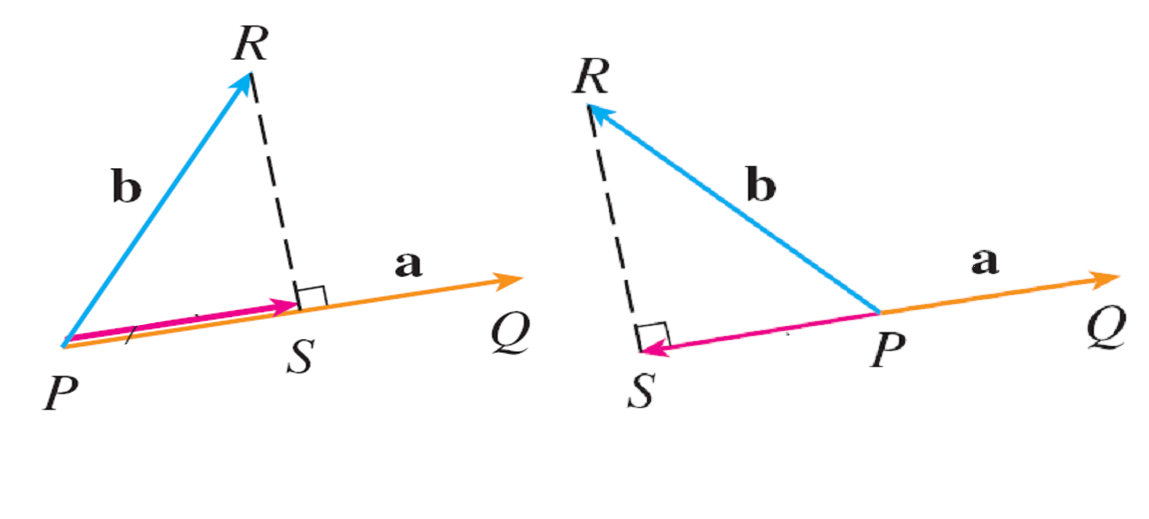
\includegraphics[width = 0.6\textwidth]{1_1.png}
\end{figure}
The vector $\overrightarrow{PS}$ is called the \textbf{vector projection} of $\ve{b}$ onto $\ve{a}$, denoted by
\[
\proj_\ve{a}\ve{b}
\]
The \textbf{scalar projection} of $\ve{b}$ onto $\ve{a}$ is defined to be the \textit{signed magnitude} of the vector projection:
\[
\comp_\ve{a}\ve{b} = \norm{\ve{b}}\cos\theta = \frac{\ve{a}\cdot\ve{b}}{\norm{\ve{a}}}
\]
Therefore,
\[
\proj_\ve{a}\ve{b}=\comp_\ve{a}\ve{b}\times\frac{\ve{a}}{\norm{\ve{a}}}=\frac{\ve{a}\cdot\ve{b}}{\ve{a}\cdot\ve{a}}\ve{a}
\]
\end{definition}
\subsection{Cross Product}
\begin{definition}[Cross Product]
\hfill\\\normalfont For two vectors $\ve{a} = \langle a_1,a_2,a_3\rangle$ and $\ve{b} = \langle b_1,b_2,b_3\rangle$, define the \textbf{cross product} of $\ve{a}$ and $\ve{b}$ to be
\[
\ve{a}\times\ve{b}=\begin{vmatrix}
                    \ve{i}&\ve{j}&\ve{k}\\
                    a_1&a_2&a_3\\
                    b_1&b_2&b_3\end{vmatrix}
\] 
\end{definition}
\begin{theorem}\normalfont The vector $\ve{a}\times\ve{b}$ is orthogonal to both $\ve{a}$ and $\ve{b}$.
\end{theorem}
The vector $\ve{a}\times\ve{b}$ points in a direction perpendicular to $\ve{a}$ and $\ve{b}$. The direction can be given by the right-hand rule.
\begin{theorem}[Cross product angle formula]
\hfill\\\normalfont If $\theta$ is the angle between $\ve{a}$ and $\ve{b}$ then
\[
\norm{\ve{a}\times\ve{b}}=\norm{\ve{a}}\norm{\ve{b}}\sin\theta
\]
\end{theorem}
\begin{theorem}[Properties of cross product]
\hfill\\\normalfont If $\ve{a},\ve{b}$ and $\ve{c}$ are vectors and $d$ a scalar, then
\begin{itemize}
  \item $\ve{a}\times\ve{b} = -\ve{b}\times\ve{a}$
  \item $(d\ve{a})\times \ve{b} = d(\ve{a}\times\ve{b})=\ve{a}\times(d\ve{b})$
  \item $\ve{a}\times(\ve{b}+\ve{c})=\ve{a}\times\ve{b}+\ve{a}\times\ve{c}$
  \item $(\ve{a}+\ve{b})\times\ve{c}=\ve{a}\times\ve{c}+\ve{b}\times\ve{c}$
\end{itemize}
\end{theorem}
\begin{theorem}
\hfill\\\normalfont Suppose two adjacent sides of a parallelogram is $\ve{a}$ and $\ve{b}$, then the height is $\norm{\ve{a}\times\ve{b}}$.\\
Suppose $Q$ is a point and $PR$ a line. The distance from $Q$ to $PR$ is
\[
\norm{\overrightarrow{PQ}}\sin\theta = \frac{\norm{\overrightarrow{PQ}\times \overrightarrow{PR}}}{\norm{\overrightarrow{PR}}}
\]
\end{theorem}
\subsection{Equation of a line}
\begin{definition}[Vector Equation of Line]
\hfill\\\normalfont
\[
\ve{r}=\ve{r}_0+t\ve{v},\;\;\;t\in\mathbb{R}
\]
is called a \textbf{vector equation} of line, where $\ve{r}_0$ is coordinate vector of a point of the line and $\ve{v}$ a direction vector of the line.
\end{definition}
\begin{theorem}[Parametric Equation of Line]
\[
x=x_0+at,\;\;\;y=y_0+bt,\;\;\;z=z_0+ct
\]
\end{theorem}
\subsection{Equation of a Plane}
\begin{theorem}[Vector Equation of Plane]
\hfill\\\normalfont
\[
\ve{n}\cdot\ve{r} = \ve{n}\cdot\ve{r}_0
\]
is a vector equation of plane, where $\ve{n}$ is the normal vector orthogonal to the plane and $\ve{r}_0$ a point on the plane.
\end{theorem}
\begin{theorem}[Linear Equation of Plane]
\hfill\\\normalfont
\[
ax+by+cz = d
\]
is the linear equation of plane, where $\langle a,b,c\rangle$ is the normal vector.
\end{theorem}
\begin{definition}[Angle between two planes]
\hfill\\\normalfont
An angle between two planes is the angle $\theta$ between their normal vectors. Notice $\pi-\theta$ is also an angle between the planes.
\end{definition}
\subsection{Vector Functions of One Variable}
\begin{definition}[Vector-valued Function]
\hfill\\\normalfont A \textbf{vector-valued function} is
\[
\ve{r}(t)=\langle f(t),g(t),h(t)\rangle = f(t)\ve{i}+g(t)\ve{j}+h(t)\ve{i}
\]
The scalar function $f,g,h$ are called the \textbf{component functions} of $\ve{r}$.
\end{definition}
The vector function $\ve{r}(t)$ traces out the curve $C$. Therefore, $\ve{r}(t)$ is a \textbf{parametrization} of $C$.
\subsection{Tangent Vectors}
\begin{definition}[Derivative of Vector-valued Functions]
\hfill\\\normalfont The \textbf{derivative} of $\ve{r}(t)$ at $t=a$ is defined by
\[
\ve{r}^\prime(a)=\Lim{\Delta t\to 0}\frac{\ve{r}(a+\Delta t)-\ve{r}(a)}{\Delta t}
\]
It can be regarded as the rate of change of $\ve{r}(t)$ at $t = a$.
\end{definition}
We also call $\ve{r}^\prime (a)$ a \textbf{tangent vector} to the curve at $t= a$.
\begin{theorem}[Derivative of Vector-valued Function]
\hfill\\\normalfont Let $\ve{r}(t) = \langle f(t),g(t),h(t)\rangle$ and suppose that the components $f,g,h$ are all differentiable at $t = a$.\\
Then $\ve{r}$ is differentiable at $t= a$ and its \textbf{derivative} is given by
\[
\ve{r}^\prime(a)= \langle f^\prime(a),g^\prime(a),h^\prime(a)\rangle
\]
\end{theorem}
\begin{theorem}[Derivative Rules]
\hfill\\\normalfont Suppose $\ve{r}(t)$ and $\ve{s}(t)$ are differentiable vector-valued functions, $f(t)$ a differentiable scalar function and $c$ is a scalar constant. Then
\begin{itemize}
  \item $\frac{\diff}{\diff t}(\ve{r}(t)+\ve{s}(t))=\ve{r}^\prime(t)+\ve{s}^\prime(t)$
  \item $\frac{\diff}{\diff t}(c\ve{r}(t))=c\ve{r}^\prime(t)$
  \item $\frac{\diff}{\diff t}f(t)\ve{r}(t)=f^\prime (t)\ve{r}(t)+f(t)\ve{r}^\prime (t)$
  \item $\frac{\diff}{\diff t}\ve{r}(t)\cdot\ve{s}(t)=\ve{r}^\prime(t)\cdot\ve{s}(t)+\ve{r}\cdot\ve{s}^\prime(t)$
  \item$\frac{\diff}{\diff t}\ve{r}(t)\times\ve{s}(t)=\ve{r}^\prime(t)\times\ve{s}(t)+\ve{r}\times\ve{s}^\prime(t)$
\end{itemize}
\end{theorem}
\clearpage
\section{Functions of Two Variables, Quadric Surfaces, Limit and Continuity}
\subsection{Two-variable function $f(x,y)$}
\begin{definition}[Two-variable function]
\hfill\\\normalfont A function $f$ of two variables is a rule that assigns, to each \textit{ordered pair} of real numbers $(x,y)$ in a set $D\subseteq \mathbb{R}^2$, a \textit{unique} real number denoted by $f(x,y)$.
\end{definition}
If a function $f$ is given by a formula and no domain is specified, then the \textbf{domain} of $f$ is understood to be\\
\fbox{
 the set of all pairs $(x, y)$ for which the given expression is a well-defined real number.

}\\
To visualise $f(x,y)$, we note that the graph of $f$ is the \textbf{surface} $S$ with equation $z=f(x,y)$.\\We can visualise the graph $S$ of $f$ lying directly above or below its domain $D$ in the $xy$-plane.\\
Visualisation can also be done through \textit{traces}.
\begin{definition}[Horizontal traces(level curves)] 
\hfill\\\normalfont \textbf{Horizontal traces} are resulting curves when we intersect the surface $z=f(x,y)$ with \textbf{horizontal} planes $z=k$.
\end{definition}
\begin{definition}[Vertical traces]
\hfill\\\normalfont \textbf{Vertical traces} are resulting curves when we intersect the surface $z=f(x,y)$ with vertical planes $x=k$ or $y=k$.
\end{definition}
\begin{definition}[Level Curve]
\hfill\\\normalfont A \textbf{level curve} of $f(x,y)$ is the \textbf{two-dimensional graph} of the equation $f(x,y)=k$ for some constant $k$.
\end{definition}
\begin{definition}[Contour Plot]
\hfill\\\normalfont A \textbf{contour plot} of $f(x,y)$ is a graph of \textbf{numerous level curves} $f(x,y)=k$, for representative values of $k$.
\end{definition}
\subsection{Cylinder and Quadric Surfaces}
\begin{definition}[Cylinders]
\hfill\\\normalfont A surface is a \textbf{cylinder} if there is a plane $P$ such that \textit{all} the planes parallel to $P$ intersect the surface in the \textit{same} curve (when viewed in 2-dimension).
\end{definition}
In fact, any equation in $x,y$ and $z$ where one of the variable is missing is a cylinder.
\begin{definition}[Quadric surface]
\hfill\\\normalfont A \textbf{quadric surface} is the graph of a \textit{second}-degree equation in three variables $x,y$ and $z$:
\[
Ax^2+By^2+Cz^2+Dxy+Eyz+Fxz+Gx+Hy+Iz+J = 0
\]
where $A, B,\ldots, J$ are constants.
\end{definition}
By translation and rotation, a quadric surface can be brought into one of the two standard forms:\\
\begin{center}
\fbox{$
Ax^2+By^2+Cz^2+J = 0\;\;\;\text{or}\;\;\;Ax^2+By^2+Iz = 0
$}
\end{center}
Excluding cylinders where one of the variable is missing, there are 6 basic quadric surfaces:
\begin{table}[h]
\centering
\begin{tabular}{|l|p{5cm}|}
\hline
Equation&\begin{minipage}{5cm}\centering Standard form\newline (symmetric about $z$-axis)\end{minipage}\\\hline
$\frac{x^2}{a^2}+\frac{y^2}{b^2}=\frac{z}{c}$&Elliptic paraboloid\\\hline
$\frac{x^2}{a^2}-\frac{y^2}{b^2}=\frac{z}{c}$&Hyperbolic paraboloid\\\hline
$\frac{x^2}{a^2}+\frac{y^2}{b^2}+\frac{z^2}{c^2}=1$&Ellipsoid\\\hline
$\frac{x^2}{a^2}+\frac{y^2}{b^2}-\frac{z^2}{c^2}=0$&Elliptic cone\\\hline
$\frac{x^2}{a^2}+\frac{y^2}{b^2}-\frac{z^2}{c^2}=1$&Hyperboloid of one sheet\\\hline
$\frac{x^2}{a^2}+\frac{y^2}{b^2}-\frac{z^2}{c^2}=-1$&Hyperboloid of two sheets\\\hline
\end{tabular}
\end{table}
\subsection{Elliptic Paraboliod}
\begin{definition}[Elliptic Paraboloid -- symmetric about the $z$-axis]
\hfill\\\normalfont 
\[
\frac{x^2}{a^2}+\frac{y^2}{b^2}=\frac{z}{c}
\]

\textbf{Horizontal} traces: Ellipses\\
\textbf{Vertical} traces: Parabolas
\begin{figure}[h]
\centering
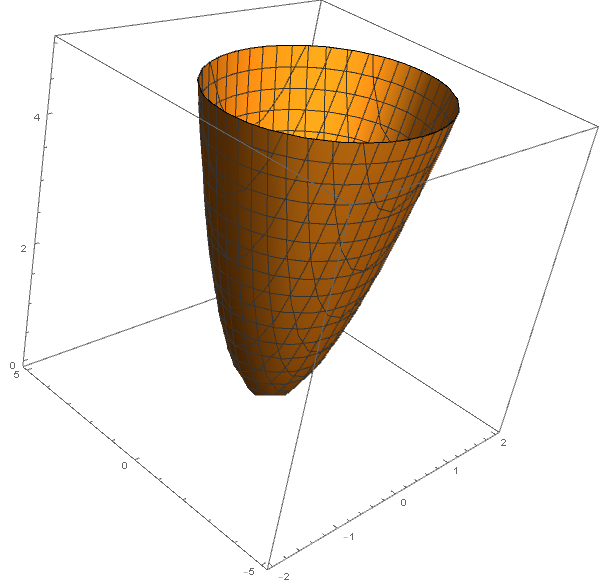
\includegraphics[width = 0.4\textwidth]{2_1.png}
\end{figure}
\end{definition} 
The point $(0,0,0)$ is called the \textbf{vertex} of the elliptic paraboloid above.\\
The vertex will e shifted to $(x_0,y_0,z_0)$ if the elliptic paraboloid is given by
\[
\frac{(x-x_0)^2}{a^2}+\frac{(y-y_0)^2}{b^2}=\frac{(z-z_0)}{c}
\]
\begin{definition}[Hyperbolic paraboloid -- symmetric about the $z$-axis]
\hfill\\\normalfont
\[
\frac{x^2}{a^2}-\frac{y^2}{b^2}=\frac{z}{c}
\]
\textbf{Horizontal} traces: Hyperbolas\\
\textbf{Vertical} traces: Parabolas
\end{definition}
\begin{figure}[h]
\centering
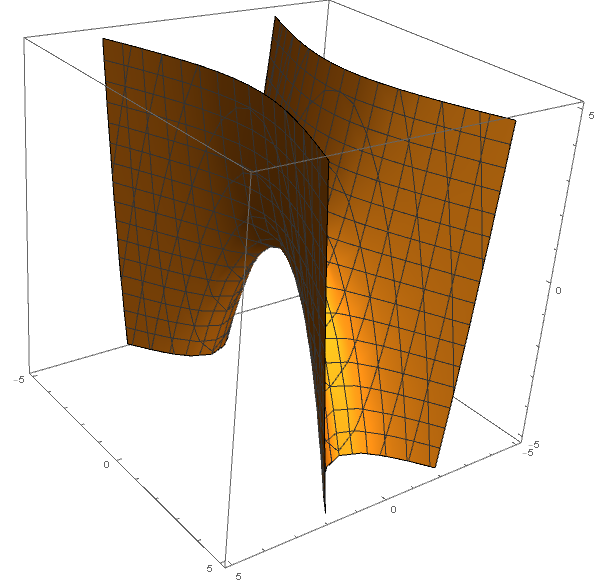
\includegraphics[width = 0.4\textwidth]{2_2.png}
\end{figure}
\subsection{Ellipsoid, Cones and Hypeboloid}
\begin{definition}[Ellipsoid]
\hfill\\\normalfont
\[
\frac{x^2}{a^2}+\frac{y^2}{b^2}+\frac{z^2}{c^2}=1
\]
\textbf{Horizontal} traces: Ellipses\\
\textbf{Vertical} traces: Ellipses
\end{definition}
\begin{figure}[h]
\centering
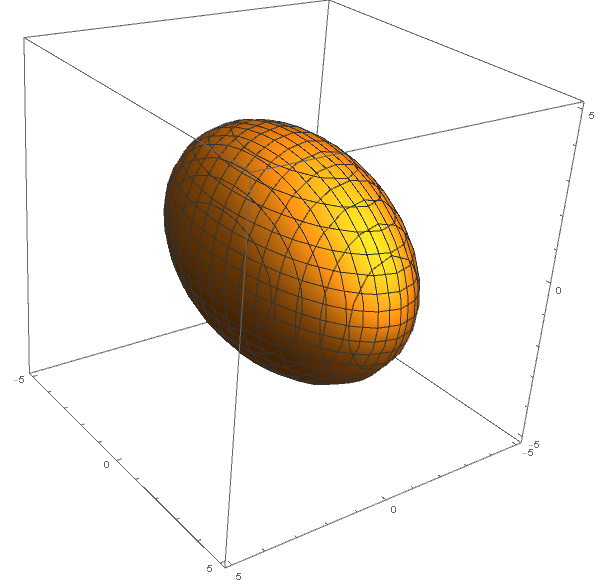
\includegraphics[width = 0.35\textwidth]{2_3.png}
\end{figure}
\begin{definition}[Elliptic cone -- symmetric about the $z$-axis]
\hfill\\\normalfont
\[
\frac{x^2}{a^2}+\frac{y^2}{b^2}-\frac{z^2}{c^2}=0
\]
\textbf{Horizontal} traces: Ellipses\\
\textbf{Vertical traces}: Hyperbolas
\end{definition}
\begin{figure}[h]
\centering
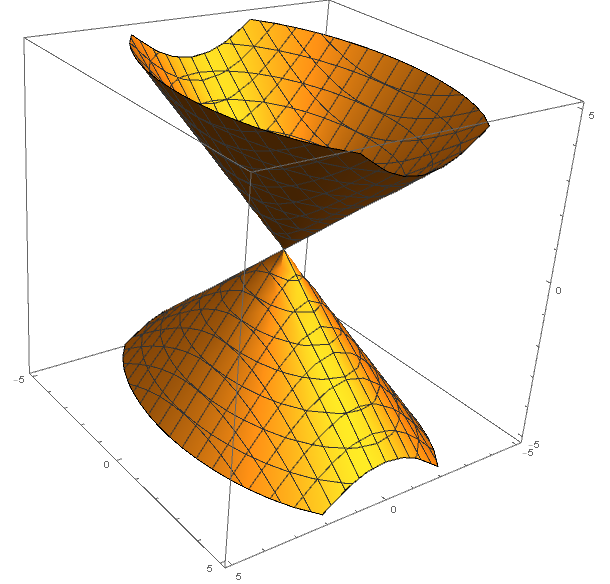
\includegraphics[width = 0.4\textwidth]{2_4.png}
\end{figure}
\begin{definition}[Hyperboloid of one sheet -- symmetric about the $z$-axis]
\hfill\\\normalfont
\[
\frac{x^2}{a^2}+\frac{y^2}{b^2}-\frac{z^2}{c^2}=1
\]
\textbf{Horizontal} traces: Ellipses\\
\textbf{Vertical traces}: Hyperbolas
\end{definition}
\begin{figure}[h]
\centering
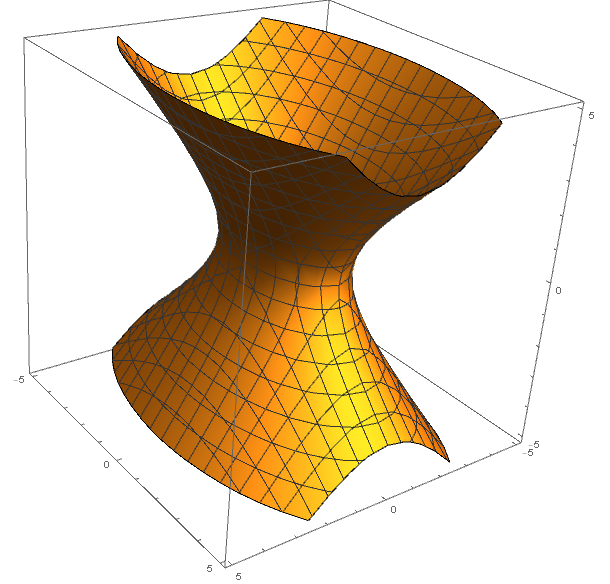
\includegraphics[width = 0.4\textwidth]{2_5.png}
\end{figure}
\begin{definition}[Hyperboloid of two sheets -- symmetric about the $z$-axis]
\hfill\\\normalfont
\[
\frac{x^2}{a^2}+\frac{y^2}{b^2}-\frac{z^2}{c^2}=-1
\]
\textbf{Horizontal} traces: Ellipses\\
\textbf{Vertical traces}: Hyperbolas
\end{definition}
\begin{figure}[h]
\centering
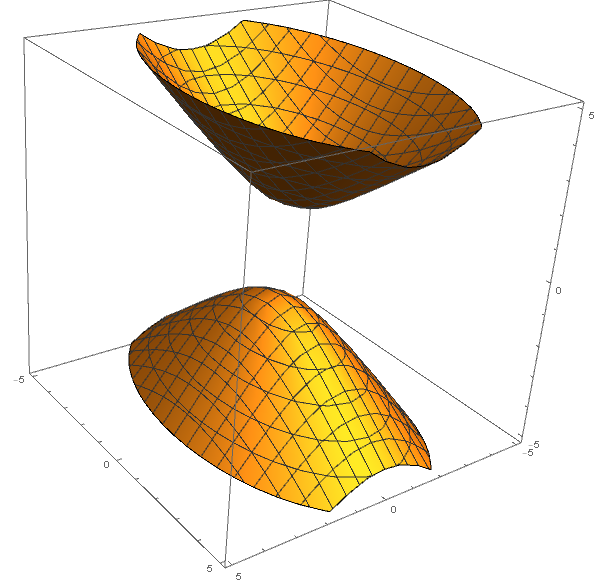
\includegraphics[width = 0.4\textwidth]{2_6.png}
\end{figure}
\subsection{Function of three Variables}
\begin{definition}\hfill\\\normalfont A function $f$ of three variables is a rule that assigns, to each \textbf{ordered triple} of real numbers $(x,y,z)$ in a set $D\subseteq \mathbb{R}^3$, a \textit{unique} real number denoted by $f(x,y,z)$.
\end{definition}
\begin{definition}[Level Surface]\hfill\\\normalfont A \textbf{level surface} of $f(x,y,z)$ is the three dimensional graph of the equation $f(x,y,z)=k$ for some constant $k$.
\end{definition}
\subsection{Limit of $f(x,y)$}
\begin{definition}[Limit]
\hfill\\\normalfont Let $f$ be a function of two variables whose domain $D$ contains points arbitrarily close to $(a,b)$. We say that the \textbf{limit} of $f(x,y)$ as $(x,y)$ approaches $(a,b)$ is $L\in\mathbb{R}$, denoted by
\[
\lim_{(x,y)\to (a,b)}f(x,y)=L
\]
if for any number $\varepsilon>0$ there exists a number $\delta>0$ such that $|f(x,y)-L|<\varepsilon$ whenever $0<\sqrt{(x-a)^2+(y-b)^2}<\delta$.
\end{definition}
\textbf{Remark}: $f$ is not required to be defined at $(a,b)$.\\
It can be proven from the definition that if $\lim_{(x,y)\to (a,b)}f(x,y)=L$, then
\begin{itemize}
  \item its value $L$ is \textit{unique}, and
  \item $L$ is \textit{independent} of the choice of path approaching $(a,b)$.
\end{itemize}
\subsection{How to show limit does not exist}
\begin{theorem}\hfill\\\normalfont If $f(x,y)$ approaches $L_1$ as $(x,y)$ approaches $(a,b)$ along a path $P_1$ and approaches $L_2$ as $(x,y)$ approaches $(a,b)$ along a path $P_2$, and $L_1\neq L_2$, then
\[
\lim_{(x,y)\to (a,b)}f(x,y)
\]
does \textbf{not} exist.
\end{theorem}
In general, some of the paths that passes through a given point $(a,b)$ to try include:
\begin{itemize}
  \item $x=a,y\to b$ (vertical lines)
  \item $y=b, x\to a$ (horizontal lines)
  \item $y=g(x), x\to a$, where $g(x)$ is some simple function (usually linear and quadratic) such that $g(a)=b$.
  \item $x=g(y), y\to b$, where $g(x)$ is some simple function (usually linear and quadratic) such that $g(b)=a$.
\end{itemize}
\subsection{How to show limit exists}
\begin{center}
\fbox{\begin{minipage}{0.7\textwidth}To show limit exists:
\begin{itemize}\item we can deduce it from known/simple functions using \textbf{properties of limit or continuity}; or\item we can use \textbf{squeeze theorem}\end{itemize}\end{minipage}}
\end{center}
\begin{theorem}[Limit Theorems]\hfill\\\normalfont Suppose $f(x,y)$ and $g(x,y)$ both have limits as $(x,y)$ approaches $(a,b)$. Then
\[
\lim_{(x,y)\to (a,b)}(f(x,y)\pm g(x,y))=\lim_{(x,y)\to (a,b)}f(x,y)\pm\lim_{(x,y)\to (a,b)}g(x,y)
\]
\[
\lim_{(x,y)\to (a,b)}f(x,y)g(x,y)=\left(\lim_{(x,y)\to (a,b)}f(x,y)\right)\left(\lim_{(x,y)\to (a,b)}g(x,y)\right)
\]
\[
\lim_{(x,y)\to (a,b)}\frac{f(x,y)}{ g(x,y)}=\frac{\lim_{(x,y)\to (a,b)}f(x,y)}{\lim_{(x,y)\to (a,b)}g(x,y)}
\]
provided
\[
\lim_{(x,y)\to (a,b)}g(x,y)\neq 0
\]
\end{theorem}
\begin{theorem}[Squeeze]\hfill\\\normalfont Suppose
\begin{itemize}
  \item $|f(x,y)-L|\leq g(x,y)\;\;\;\forall (x,y)\text{ close to }(a,b)$
  \item $\lim_{(x,y)\to (a,b)}g(x,y)=0$
\end{itemize}
Then,
\[
\lim_{(x,y)\to (a,b)}f(x,y)=L
\]
\end{theorem}
\subsection{Continuity of $f(x,y)$}
\begin{definition}[Continuity]\hfill\\\normalfont We say $f$ is \textbf{continuous at} $(a,b)$ if
\[
\lim_{(x,y)\to (a,b)}f(x,y)=f(a,b)
\]
\end{definition}
\begin{theorem}[Continuity Theorems]\hfill\\\normalfont If $f(x,y)$ and $g(x,y)$ are continuous at $(a,b)$, then
\begin{itemize}
  \item $f\pm g$ is continuous at $(a,b)$.
  \item $f\cdot g$ is continuous at $(a,b)$.
  \item $\frac{f}{g}$ is continuous at $(a,b)$, provided $g(a,b)\neq 0$.
\end{itemize}
\end{theorem}
\begin{theorem}[Continuity of Composite Function]
\hfill\\\normalfont Suppose $f(x,y)$ is continuous at $(a,b)$ and $g(x)$ is continuous at $f(a,b)$. Then
\[
h(x,y)=(g\circ f)(x,y)=g(f(x,y))
\]
is continuous at $(a,b)$.
\end{theorem}
Subsequently, the following classes of functions are continuous \textbf{in its domain}.
\begin{itemize}
  \item Polynomial in $x$ and $y$.
  \item Trigonometric and exponential functions in $x$ and $y$.
  \item Rational function in $x$ and $y$.
\end{itemize}
\clearpage
\section{Partial Derivatives, Chain Rule, Directional Derivatives}
\subsection{Partial Derivative}
\begin{definition}[Partial Derivative]
\hfill\\\normalfont If $f$ is a function of two variables, its \textbf{partial derivatives} are the functions $f_x$ and $f_y$ defined by: 
\begin{align*}
f_x(x,y)&=\lim_{h=0}\frac{f(x+h,y)-f(x,y)}{h}\\
f_y(x,y)&=\lim_{h=0}\frac{f(x,y+h)-f(x,y)}{h}
\end{align*}
\end{definition}
Other notations for partial derivatives:
\[
f_x=\frac{\partial f}{\partial x}\;\;\;f_y=\frac{\partial f}{\partial y}
\]
\subsection{Higher Order Partial Derivatives}
\begin{definition}[Second partial derivatives]
\hfill\\\normalfont Second partial derivatives of $f$ is the partial derivatives of partial derivatives of $f$, i.e.
\[
(f_x)_x,(f_x)_y,(f_y)_x,(f_y)_y
\]
\end{definition}
We use the following notation:
\begin{alignat*}{2}
(f_x)_x&=f_{xx}&=\frac{\partial^2 f}{\partial x^2}\\
(f_x)_y&=f_{xy}&=\frac{\partial^2 f}{\partial y\partial x}\\
(f_y)_x&=f_{yx}&=\frac{\partial^2 f}{\partial x\partial y}\\
(f_y)_y&=f_{yy}&=\frac{\partial^2 f}{\partial y^2}
\end{alignat*}
Thus, the notation $f_{xy}$ means that we \textit{first} differentiate with respect to $x$ and \textit{then} with respect to $y$.
\begin{theorem}[Clairaut's Theorem]
\hfill\\\normalfont Suppose $f$ is defined on a disk $D$ that contains $(a,b)$. If the functions $f_{xy}$ and $f_{yx}$ are both \textit{continuous} on $D$, then
\[
f_{xy}(a,b)=f_{yx}(a,b)
\]
\end{theorem}
In fact, so long as the number of the same variable occurring in the subscript are the same, the coresponding partial derivatives are the same.
\subsection{Tangent Plane Equation}
\begin{definition}[Tangent Plane]
\hfill\\\normalfont The \textbf{tangent plane} to the surface $S$ at the point $P(a,b,c)$ is defined to be the plane that contains both tangent lines $T_1$ and $T_2$, where $T_1$ and $T_2$ are the tangent lines to the curves of intersections of the surface $S$ and the vertical planes $y=b$ and $x=a$ respectively.
\begin{figure}[h]
\centering
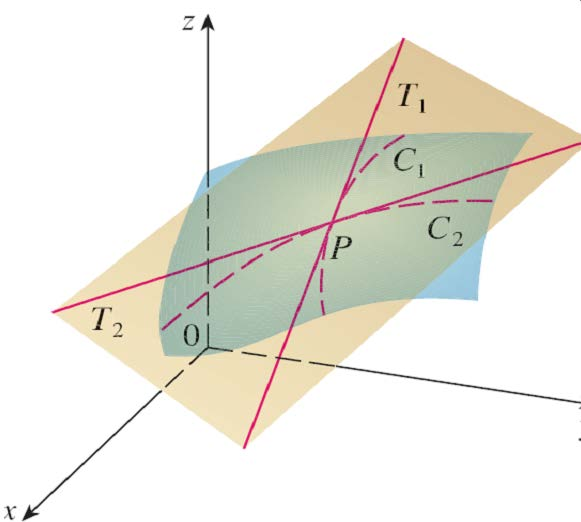
\includegraphics[width = 0.5\textwidth]{3_1.jpg}
\end{figure}
\end{definition}
From the definition, we note that two vectors on the tangent plane are $\langle 1,0,f_x(a,b)\rangle$ and $\langle 0,1,f_y(a,b)\rangle$. Thus, a normal vector to the plane is
\[
\ve{n}=\langle f_x(a,b),f_y(a,b),-1\rangle
\]
\begin{theorem}[Equation of Tangent Plane]
\hfill\\\normalfont Consider the surface $S$ given by $z=f(x,y)$. A normal vector to the tangent plane to $S$ at $(a,b)$ is
\[\langle f_x(a,b),f_y(a,b),-1\rangle\]
The tangent plane is given by
\[
\langle x-a,y-b,z-f(a,b)\rangle \cdot \langle f_x(a,b),f_y(a,b),-1\rangle = 0
\]
Equivalently,
\[
z=f(a,b)+f_x(a,b)(x-a)+f_y(a,b)(y-b)
\]
\end{theorem}
\subsection{Differentiability of $f(x,y)$}
In general, for $f(x,y)$ we have
\begin{center}
\fbox{$f$ differentiable $\Rightarrow$ $f_x$ and $f_y$ exist} 
\end{center}
To define differentiability, we first define \textbf{increment}.
\begin{definition}[Increment]\hfill\\\normalfont Let $z=f(x,y)$. Suppose $\Delta x$ and $\Delta y$ are increments in the \textit{independent} variable $x$ and $y$ respectively from a fixed point $(a,b)$. Then the \textbf{increment} in $z$ at $(a,b)$, $\Delta z$, is defined by
\[
\Delta z = f(a+\Delta x, b+\Delta y)-f(a,b)
\]
\end{definition}
\begin{definition}[Differentiability - Two Variable]
\hfill\\\normalfont Let $z=f(x,y)$. We say that $f$ is \textbf{differentiable} at $(a,b)$ if we can write
\[
\Delta z = f_x(a,b)\Delta x+f_y(a,b)\Delta y+\epsilon_1\Delta x + \epsilon_2\Delta y
\]
where $\epsilon_1$ and $\epsilon_2$ are functions of $\Delta x$ and $\Delta y$ which vanish (i.e. $\epsilon_1,\epsilon_2\to 0$ as $(\Delta x,\Delta y)\to(0,0)$).\footnote{Rearranging $\Delta z = (f_x(a,b)+\epsilon_1)\Delta x+(f_y(a,b)+\epsilon_2)\Delta y$, we will see the function is differentiable if the directional derivative at $(a,b,f(a,b))$ is will estimated in all direction when $\Delta x,\Delta y)\to 0$, which suggests that the tangent vector in all direction at $(a,b,f(a,b))$ will contain in the tangent plane.}
\end{definition}
We say that $f$ is \textbf{differentiable on a region} $R\in\mathbb{R}^2$ if $f$ is differentiable at every point in $R$.
\subsection{Linear Approximation}
\begin{theorem}[Linear Approximation - Two Variable]
\hfill\\\normalfont Suppose $z=f(x,y)$ is \textit{differentiable} at $(a,b)$. Let $\Delta x$ and $\Delta y$ be small increments in $x$ and $y$ respectively from $(a,b)$. Then
\[
\Delta z \approx f_x(a,b)\Delta x+f_y(a,b)\Delta y
\]
\end{theorem}
This result can be extended to functions of more variables.
\subsection{Chain Rule}
\begin{theorem}[Chain Rule - Case 1]
\hfill\\\normalfont Suppose that $z=f(x,y)$ is a \textit{differentiable} function of $x$ and $y$, where $x=g(t)$ and $y=h(t)$ are both \textit{differentiable} functions of $t$. Then, $z$ is a \textbf{differentiable} function of $t$ and
\[
\frac{\diff z}{\diff t}=\frac{\partial f}{\partial x}\frac{\diff x}{\diff t}+\frac{\partial f}{\partial y}\frac{\diff y}{\diff t}
\] 
\end{theorem}
\begin{theorem}[Chain Rule - Case 2]
\hfill\\\normalfont Suppose that $z=f(x,y)$ is a \textit{differentiable} function of $x$ and $y$, where $x=g(s,t)$ and $y=h(s,t)$ are both \textit{differentiable} functions of $s$ and $t$. Then, $z$ is a \textbf{differentiable} function of $s$ and $t$ and
\[
\frac{\partial z}{\partial t}=\frac{\partial f}{\partial x}\frac{\partial x}{\partial t}+\frac{\partial f}{\partial y}\frac{\partial y}{\partial t}
\] 
\end{theorem}
Here there are three types of variables:
\begin{itemize}
  \item $s$ and $t$ are \textbf{independent} variables.
  \item $x$ and $y$ are called \textbf{intermediate} variables.
  \item $z$ is the \textbf{dependent} variable.
\end{itemize}
\begin{theorem}[Chain Rule - General Version]
\hfill\\\normalfont Suppose that $u$ is a differentiable function of $n$ variables $x_1,\ldots, x_n$, and each $x_j$ is a differentiable function of $m$ variables $t_1,\ldots ,t_m$. Then $u$ is a function of $t_1,\ldots, t_m$ and
\[
\frac{\partial u}{\partial t_i}=\frac{\partial u}{\partial x_1}\frac{\partial x_1}{\partial t_i}+\cdots+\frac{\partial u}{\partial x_n}\frac{\partial x_n}{\partial t_i}
\]
\end{theorem}
\subsection{Implicit Differentiation}
\begin{definition}[Implicit Function]
\hfill\\\normalfont $z$ is an \textbf{implicit function} of $x$ and $y$ defined by $F(x,y,z)=0$ if
\begin{center}
\fbox{\begin{minipage}{0.7\textwidth}for every choice of $x$ and $y$, the value of $z$ is determined by $F(x,y,z)=0$\end{minipage}}
\end{center}
\end{definition}
\begin{theorem}[Implicit Differentiation: Two Independent Variables]
\hfill\\\normalfont Suppose the equation $F(x,y,z)=0$, where $F$ is \textit{differentiable}, defines $z$ \textbf{implicitly} as a differentiable function of $x$ and $y$. Then,
\[
\frac{\partial z}{\partial x}=-\frac{F_x(x,y,z)}{F_z(x,y,z)},\;\;\;\frac{\partial z}{\partial y}=-\frac{F_y(x,y,z)}{F_z(x,y,z)}
\]
provided $F_z(x,y,z)\neq 0$.
\end{theorem}
\subsection{Directional Derivatives}
\begin{definition}[Directional Derivative]
\hfill\\\normalfont The \textbf{directional derivative} of $f(x,y)$ at $(x_0,y_0)$ in the direction of \textbf{unit} vector $\ve{u}=\langle a,b\rangle$ is
\[
D_\ve{u}f(x_0,y_0) = \lim_{h\to 0}\frac{f(x_0+ha,y_0+hb)-f(x_0,y_0)}{h}
\]
\end{definition}
The idea of directional derivative can be extended to functions of more variables.
\begin{theorem}[Computing Directional Derivatives]
\hfill\\\normalfont If $f(x,y)$ is a \textit{differentiable} function, then $f$ has a directional derivative in the direction of any unit vector $\ve{u}=\langle a,b\rangle$ and
\[
D_\ve{u}f(x_0,y_0)=\langle a,b\rangle \cdot \ve{u}
\]
\end{theorem}
\begin{definition}[Gradient]
\hfill\\\normalfont The \textbf{gradient} of $f(x,y)$ is the vector-valued function
\[
\nabla f(x,y) = \langle f_x,f_y\rangle
\]
provided that both partial derivatives exist.
\end{definition}
\clearpage
\section{Gradient Vector, Extrema, Langrange Multiplier}
\subsection{Gradient Vector and Level Curve}
\begin{theorem}[Level Curve vs $\nabla f$]
\hfill\\\normalfont Suppose $f(x,y)$ is differentiable function of $x$ and $y$ at $(x_0,y_0)$. Suppose $\nabla f(x_0,y_0)\neq \ve{0}$\\
Then $\nabla f(x_0,y_0)$ is \textbf{normal} to the level curve $f(x,y)=k$ that contains the point $(x_0,y_0)$.
\end{theorem}
\subsection{Gradient Vector and Level Surface}
\begin{theorem}[Level Surface vs $\nabla F$]
\hfill\\\normalfont Suppose $F(x,y,z)$ is diffeerentiable function of $x$, $y$ and $z$ at $(x_0,y_0,z_0)$. Suppose $\nabla F(x_0,y_0,z_0)\neq \ve{0}$.\\
Then $\nabla F(x_0,y_0,z_0)$ is \textbf{normal} to the level surface $F(x,y,z)=k$ that contains the point $(x_0,y_0,z_0)$.
\end{theorem}
\begin{theorem}[Tangent Plane to Level Surface]
\hfill\\\normalfont The tangent plane to the level surface $F(x,y,z)=k$ on which $(x_0,y_0,z_0)$ resides is given by
\[
\nabla F(x_0,y_0,z_0)\cdot\langle x-x_0,y-y_0,z-z_0\rangle = 0
\]
\end{theorem}
\subsection{Maximum/Minimum Rate of Change}
At a given point $(x_0,y_0,z_0)$, the rate of change of $f(x,y,z)$ is given by
\begin{align*}
D_\ve{u}f&=\nabla f\cdot\ve{u}\\
&=\norm{\nabla f}\norm{\ve{u}}\cos\theta\\
&=\norm{\nabla}\cos\theta
\end{align*}
where $\theta$ is the ange between $\nabla f$ and $\ve{u}$.
\begin{theorem}[Maximising rate of Increase/Decrease of $f$]
\hfill\\\normalfont Suppose $f$ is a differentiable function of two or three variables. Let $P$ denote a given point. Assume $\nabla f(P)\neq \ve{0}$.
\begin{itemize}
  \item $\nabla f(P)$ points in the direction of maximum rate of change of $f$ at $P$,$\norm{\nabla f(P)}$.
  \item $-\nabla f(P)$ points in the direction of minimum rate of change of $f$ at $P$,$-\norm{\nabla f(P)}$.
\end{itemize}
\end{theorem}
\subsection{Critical Points of $f(x,y)$}
\begin{definition}[Local Maximum]
\hfill\\\normalfont Let $f(x,y):D\to\mathbb{R}$. Then $f$ has a \textbf{local maximum} at $(a,b)$ if
\[
f(x,y)\leq f(a,b) \text{for all points close to }(a,b)
\]
The number $f(a,b)$ is called a local maximum value.
\end{definition}
\begin{definition}[Local Minimum]
\hfill\\\normalfont Let $f(x,y):D\to\mathbb{R}$. Then $f$ has a \textbf{local minimum} at $(a,b)$ if
\[
f(x,y)\geq f(a,b) \text{for all points close to }(a,b)
\]
The number $f(a,b)$ is called a local minimum value.
\end{definition}
\begin{theorem}[A necessary condition]
\hfill\\\normalfont If $f$ has a local maximum or minimum at $(a,b)$ and the first-order derivatives of $f$ exist there, then
\[
f_x(a,b)=f_y(a,b)=0
\]
\end{theorem}
\begin{definition}[Saddle Point]
\hfill\\\normalfont Let $f(x,y):D\to\mathbb{R}$. Then a point $(a,b)$ is called a \textbf{saddle point} of $f$ if
\begin{enumerate}
  \item $f_x(a,b)=f_y(a,b)=0$; and
  \item every neighbourhood at $(a,b)$ contains points $(x,y)\in D$ for which $f(x,y)<f(a,b)$ and points $(x,y)\in D$ for which $f(x,y)>f(a,b)$.
\end{enumerate}
\end{definition}
\subsection{Finding Absolute Maximum/Minimum}
\begin{definition}[Absolute Maximum]
\hfill\\\normalfont Let $f(x,y):D\to\mathbb{R}$. Then $f$ has an \textbf{absolute maximum} at $(a,b)$ if
\[
f(x,y)\leq f(a,b)\text{ for all points in the domain }D
\]
The number $f(a,b)$ is called a \textbf{absolute maximum value}.
\end{definition}
\begin{definition}[Absolute Minimum]
\hfill\\\normalfont Let $f(x,y):D\to\mathbb{R}$. Then $f$ has an \textbf{absolute minimum} at $(a,b)$ if
\[
f(x,y)\geq f(a,b)\text{ for all points in the domain }D
\]
The number $f(a,b)$ is called a \textbf{absolute minimum value}.
\end{definition}
\begin{definition}[Closed Set in $\mathbb{R}^2$]
\hfill\\\normalfont A set $R\subseteq\mathbb{R}^2$ is \textbf{closed} if it contains all its boundary points.\\
A \textbf{boundary point} of $R$ is a point $(a,b)$ such that every disk with center $(a,b)$ contains point in $R$ and also points in $\mathbb{R}^2\setminus R$.
\end{definition}
\begin{definition}[Bounded Set in $\mathbb{R}^2$]
\hfill\\\normalfont A set $R\subseteq\mathbb{R}^2$ is \textbf{bounded} if it is contained within some disk. In other words, it is finite in extent.
\end{definition}
\begin{theorem}[Extreme Value Theorem]
\hfill\\\normalfont If $f(x,y)$ is continuous on a closed and bounded set $D\subseteq \mathbb{R}^2$, then $f$ attains
\begin{itemize}
  \item an absolute maximum value $f(x_1,y_1)$ and
  \item an absolute minimum value $f(x_2,y_2)$
\end{itemize}
at some points $(x_1,y_1)$ and $(x_2,y_2)$ in $D$.
\end{theorem}
\begin{theorem}[Closed Interval Method]
\hfill\\\normalfont
The following is the \textbf{closed interval method} for finding absolute maximum and minimum
\begin{itemize}
  \item[Step 1] Find the values of $f$ at its \textbf{critical points} in $D$.
  \item[Step 2] Find the extreme values of $f$ on the \textbf{boundary} of $D$.
  \item[Step 3] The \textbf{largest}(resp. \textbf{smallest}) of the values from \textbf{Step 1} and \textbf{Step 2} is the \textbf{absolute maximum}(resp. \textbf{absolute minimum}).
\end{itemize}
\end{theorem}
\subsection{Lagrange Multiplier -- 2-Variable Case}
\begin{theorem}[Lagrange Multipliers for Function of Two Variables]
\hfill\\\normalfont Suppose $f(x,y)$ and $g(x,y)$ are differentiable functions such that $\nabla g(x,y)\neq \ve{0}$ on the constraint curve $g(x,y)=k$.\\
Suppose that the \textbf{minimum}/\textbf{maximum} value of $f(x,y)$ subject to the constraint $g(x,y)=k$ occurs at $(x_0,y_0)$. Then
\[
\nabla f(x_0,y_0)=\lambda\nabla g(x_0,y_0)
\]
for some constant $\lambda$.\\
The following are the steps of the method of Lagrange Multiplier for two variable functions:
\begin{itemize}
  \item[Step 1] Find all values of $x,y$ and $\lambda$ such that
  \[
  \nabla f(x,y)=\lambda\nabla g(x,y)
  \]
  and
  \[
g(x,y)=k
  \]
  \item[Step 2] Evaluate $f$ at all points obtained in \textbf{Step 1}.
  \begin{itemize}
    \item The largest of these values is the maximum value of $f$;
    \item The smallest is the minimum value of $f$.
  \end{itemize}
\end{itemize}
\end{theorem}
This theorem can be extended to functions of three variables.
\clearpage
\section{Double Integral over region on the $xy$--plane}
\begin{definition}[Double Integral over Rectangle]
\hfill\\\normalfont The \textbf{double integral} of $f$ over the \textbf{rectangle} $R$ is
\[
\iint_Rf(x,y)\diff A = \lim_{m,n\to\infty}\sum_{i=1}^m\sum_{j=1}^n f(x_{ij}^\ast,y_{ij}^\ast)\Delta A
\] 
provided that the limit exists and is the same for any choice of the sample points $(x_{ij}^\ast, y_{ij}^\ast)$ in $R_{ij}:=[x_{i-1},x_i]\times[y_{j-1},y_j]$ whose region is $\Delta A = \Delta x\times\Delta y$, for $1\leq i\leq m, 1\leq j\leq n$.
\end{definition}
\begin{definition}[Double Integral over General Region]
\hfill\\\normalfont \textbf{Double integral} of $f$ over general region $D$ is defined by
\[
\iint_D f(x,y)\diff A = \iint_R F(x,y)\diff A
\] 
where 
\[
F(x,y)=\begin{cases}f(x,y)&\text{ if }(x,y)\in D\\0&\text{ if }(x,y)\in R\setminus D\end{cases}
\]
\end{definition}
Double integrals are computed by means of iterated integrals.
\begin{definition}[Iterated Integral]
\hfill\\\normalfont The \textbf{iterated double integral} of $f$ on the rectangle $R = [a,b]\times[c,d]$ in the \textbf{order} $\diff y\diff x$ is defined to be
\[
\int_a^b\left(\int_c^df(x,y)\diff y\right)\diff x
\] 
The \textbf{iterated double integral} of $f$ on the rectangle $R = [a,b]\times[c,d]$ in the \textbf{order} $\diff x\diff y$ is defined to be
\[
\int_c^d\left(\int_a^bf(x,y)\diff x\right)\diff y
\] 
\end{definition}
\begin{theorem}[Fubini's Theorem]
\hfill\\\normalfont If $f$ is \textbf{continuous} on the rectangle $R=[a,b]\times[c,d]$, then
\[
\iint_R f(x,y)\diff A = \int_a^b\int_c^df(x,y)\diff y\diff x =\int_c^d(\int_a^bf(x,y)\diff x\diff y
\]
\end{theorem}
\begin{definition}[Type I Region]
\hfill\\\normalfont A plane region $D$ is said to be of \textbf{Type I} if it lies between the graphs of two continuous functions of $x$, that is
\[
D=\{(x,y)\mid a\leq x\leq b, g_1(x)\leq y\leq g_2(x)\}
\]
where $g_1(x)$ and $g_2(x)$ are continuous on $[a,b]$.
\end{definition}
\begin{definition}[Type II Region]
\hfill\\\normalfont A plane region $D$ is said to be of \textbf{Type II} if it lies between the graphs of two continuous functions of $y$, that is
\[
D=\{(x,y)\mid c\leq y\leq d, h_1(y)\leq x\leq h_2(y)\}
\]
where $h_1(y)$ and $h_2(y)$ are continuous on $[c,d]$.
\end{definition}
\begin{theorem}[Double Integral over Type I Domain]
\hfill\\\normalfont If $f$ is continuous on a \textbf{Type I} domain $D$ such that
\[
D=\{(x,y)\mid a\leq x\leq b, g_1(x)\leq y\leq g_2(x)\}
\]
then
\[
\iint_D f(x,y)\diff A = \int_a^b\int_{g_1(x)}^{g_2(x)} f(x,y)\diff y\diff x
\]
\end{theorem}
\begin{theorem}[Double Integral over Type II Domain]
\hfill\\\normalfont If $f$ is continuous on a \textbf{Type II} domain $D$ such that
\[
D=\{(x,y)\mid c\leq y\leq d, h_1(y)\leq x\leq h_2(y)\}
\]
then
\[
\iint_D f(x,y)\diff A = \int_c^d\int_{h_1(y)}^{h_2(y)} f(x,y)\diff x\diff y
\]
\end{theorem}
\begin{theorem}[Additivity with respect to Domain]
\hfill\\\normalfont 
\[
\iint_D f(x,y)\diff A = \sum_{i=1}^n\iint_{D_i}f(x,y)\diff A
\]
\end{theorem}
The theorem above allows us to decompose the domain into finitely many domains of Type I or II.
\clearpage
\section{Double Integral over Polar Regions and Triple Integrals}
\begin{theorem}[Relationship between polar coordinates $(r,\theta)$ and cartesian coordinates $(x,y)$]
\[
x = r\cos\theta \;\;\; y = r\sin\theta
\]
\[r = \sqrt{x^2+y^2}\;\;\; \theta = \tan^{-1}\frac{y}{x},\text{ provided }x\neq 0
\]
\end{theorem}
\begin{definition}[Polar Rectangle]
\hfill\\\normalfont A polar rectangle is a region
\[
R=\{(r,\theta): a\leq r\leq b, \alpha\leq \theta\leq \beta\}
\]
\end{definition}
\begin{theorem}[Change to Polar Coordinates in Double Integrals]
\hfill\\\normalfont If $f$ is continuous on a polar rectangle $R$ given by
\[
R=\{(r,\theta): 0\leq a\leq r\leq b,\alpha\leq\theta\leq \beta\}
\]
where $0\leq \beta-\alpha\leq 2\pi$, then
\[
\iint_R f(x,y)\diff A = \int_\alpha^\beta\int_a^b f(r\cos\theta, r\sin\theta)r\diff r\diff \theta
\]
\end{theorem}
\begin{definition}[General Polar Regions]
\hfill\\\normalfont General polar regions come in two different forms:
\[
D_1=\{(r,\theta): a\leq r\leq b, g_1(r)\leq \theta\leq g_2(r)\}
\]
or
\[
D_2=\{(r,\theta): \alpha\leq \theta\leq \beta, h_1(\theta)\leq r\leq h_2(\theta)\}
\]
\end{definition}
\begin{theorem}\hfill\\\normalfont If $f$ is continuous on a polar regions $D_1$, then
\[
\iint_D f(x,y)\diff A = \int_a^b\int_{g_1(r)}^{g_2(r)} f(r\cos\theta,r\sin\theta)r\diff\theta\diff r
\]
If $f$ is continuous on a polar region $D_2$, then
\[
\iint_D f(x,y)\diff A = \int_\alpha^\beta\int_{h_1(\theta)}^{h_2(\theta)} f(r\cos\theta,r\sin\theta)r\diff r\diff \theta
\]
\end{theorem}
\begin{definition}[Rectangular box]
\hfill\\\normalfont A rectangular box is defined by
\[
B=\{(x,y,z):a\leq x\leq b, c\leq y\leq d, r\leq z\leq s\}
\]
\end{definition}
\begin{theorem}[Fubini's Theorem for Triple Integral]
\hfill\\\normalfont If $f$ is continuous on the rectangular box $B$, then
\[
\iiint_B f(x,y,z)\diff V = \int_r^s\int_c^d\int_a^b f(x,y,z)\diff x\diff y\diff z
\]
Furthermore, the iterated integral may be evaluated in any order.
\end{theorem}
\clearpage
\section{Line Integrals}
\subsection{Line Integral of Scalar Field}
\begin{definition}[Line Integrals of Scalar Field]\hfill\\\normalfont If $f$ is defined on a smooth curve $C$ given by $\mathbf{r}(t) = \langle x(t),y(t)\rangle , a\leq t\leq b$. Then the \textbf{line integral} of $f$ along $C$ is
\[
\int_Cf(x,y)\diff s = \lim_{n\to\infty}\sum_{i=1}^n f(x_i^\ast, y_i^\ast)\Delta s_i
\]
provided this limit exists and is the same for every choice of $(x_i^\ast, y_i^\ast)$.
\end{definition}
\begin{theorem}[Formula for evaluation of Line Integral of Scalar Field]
\hfill\\\normalfont Suppose $C$ is given by $\mathbf{r}(t) = \langle x(t),y(t)\rangle, a\leq t\leq b$, then
\begin{align*}
\int_Cf(x,y)\diff s &= \int_a^bf(x(t),y(t))\norm{\mathbf{r}^\prime(t)}\diff t\\
&=\int_a^bf(x(t),y(t))\sqrt{\left(\frac{\diff x}{\diff t}\right)^2+\left(\frac{\diff y}{\diff t}\right)^2}\diff t
\end{align*}
Similarly, suppose that $C$ is smooth space curve given by $\mathbf{r}(t)=\langle x(t),y(t),z(t)\rangle, a\leq t\leq b$. Then
\begin{align*}
\int_C f(x,y,z)\diff s &=\int_a^b f(x(t),y(t),z(t))\norm{\mathbf{r}^\prime(t)}\diff t\\
&=\int_C f(x(t),y(t),z(t))\sqrt{\left(\frac{\diff x}{\diff t}\right)^2+\left(\frac{\diff y}{\diff t}\right)^2+\left(\frac{\diff z}{\diff t}\right)^2}\diff t
\end{align*}
\end{theorem}
\textbf{Remark:} If $f(x,y)=1$ for all $x,y$, the line integral formula evaluates the \textbf{arc length} of $C$.\\
More generally, one can interpret the line integral $\int_Cf(x,y)\diff s$ as the \textbf{area} of the fence, whose base is $C$ and height above the point $(x,y)$ is $f(x,y)$.
\begin{theorem}[Piecewise Parametrisation]
\hfill\\\normalfont Suppose $C$ is a union of a finite number of smooth curves $C_1, C_2,\ldots, C_n$, where the initial point of $C_{i+1}$ is the terminal point of $C_i$. Then
\[
\int_Cf(x,y)\diff s = \sum_{i=1}^n \int_{C_i}f(x,y)\diff s
\]
\end{theorem}
\begin{theorem}[Parametrisation of Line Segment]
\hfill\\\normalfont A vector parametrisation of line segment that starts from $\mathbf{r}_0$ and ends at $\mathbf{r}_i$ is given by
\[
\mathbf{r}(t) = \mathbf{r}_0+t(\mathbf{r}_1-\mathbf{r}_0),\;\;\;\;\;0\leq t\leq 1
\]
\end{theorem}
\subsection{Vector Field}
\begin{definition}[Vector field]
Let $D\subseteq \mathbb{R}^2$. A \textbf{vector field} on $D$ is a function $\mathbf{F}$ that assigns to each point $(x,y)\in D$ a 2D vector $\mathbf{F}(x,y)$.\\
Let $D\subseteq \mathbb{R}^3$. A \textbf{vector field} on $D$ is a function $\mathbf{F}$ that assigns to each point $(x,y,z)\in D$ a 3D vector $\mathbf{F}(x,y,z)$.
\end{definition}
\begin{theorem}[Vector Field in Component Form]
\hfill\\\normalfont For vector field $\mathbf{F}$ on $\mathbb{R}^2$,
\[
\mathbf{F}(x,y) = P(x,y)\mathbf{i}+Q(x,y)\mathbf{j} = \langle P(x,y),Q(x,y)\rangle
\]
or for short
\[
\mathbf{F} = \langle P,Q\rangle
\]
Similarly, for vector field on $\mathbf{F}$ on $\mathbb{R}^3$,
\[
\mathbf{F} = \langle P,Q,R\rangle
\]
\end{theorem}
\begin{definition}[Line Integral of Vector Field]
\hfill\\\normalfont Let $\mathbf{F}$ be a continuous vector field defined on a smooth curve $C$ given by a vector function $\mathbf{r}(t) = \langle x(t),y(t),z(t)\rangle, a\leq t\leq b$. \\Then, the \textbf{line integral} of $\mathbf{F}(x,y,z)$ along $C$ is
\[
\int_C\mathbf{F}\cdot \diff\mathbf{r} :=\int_C\mathbf{F}\cdot\mathbf{T}\diff s = \int_a^b \mathbf{F}(x(t),y(t),z(t))\cdot \mathbf{r}^\prime(t)\diff t
\]
\end{definition}
\begin{theorem}\hfill\\\normalfont We have
\[
\int_{-C}\mathbf{F}\cdot\diff \mathbf{r} = -\int_C\mathbf{F}\cdot\diff\mathbf{r}
\]
\end{theorem}
\begin{theorem}[Component Form]
\hfill\\\normalfont If $\mathbf{F}(x,y,z)=\langle P,Q,R\rangle$ then we have
\[
\int_C\mathbf{F}\cdot\diff\mathbf{r} = \int_C P\diff x+Q\diff y+R\diff z
\]
Sometimes a curve $C$ is a union of finitely many smooth curves $C_1,\ldots, C_n$. In such cases,
\[
\int_C \mathbf{F}\cdot\diff\mathbf{r} = \sum_{i=1}^n\int_{C_i}\mathbf{F}\cdot\diff\mathbf{r}
\]
\end{theorem}
\subsection{Conservative Vector Field}
\begin{definition}[Conservative Vector Field]
\hfill\\\normalfont A vector field $\mathbf{F}$ is \textbf{conservative vector field} on $D$ if we can write
\[
\mathbf{F}= \nabla f
\]
for some scalar function $f$ on $D$.
\end{definition}
The function $f$ is called the \textbf{potential function} of $\mathbf{F}$.
\begin{theorem}[Recovering {$f$} from {$\mathbf{F}$}]\hfill\\\normalfont
\begin{itemize}
  \item Suppose $\mathbf{F} = \langle P,Q\rangle$, we have $f_x = P, f_y = Q$.
  \item Integrating $f_x$ with respect to $x$, we have
  \[
f(x,y) = j(x,y)+h(y)
  \]
  where $\frac{\partial}{\partial x}j(x,y) = f_x$.
  \item Differentiate $f(x,y)$ with respect to $y$, we have
  \[
f_y = \frac{\partial }{\partial y}j(x,y)+h^\prime(y)
  \]
  and by comparing the above expression with $Q$, we have\[g^\prime(y) = Q-\frac{\partial }{\partial y}j(x,y)\]
  \item Integrating $g^\prime(y)$ with respect to $y$, we will have $g(y)$, which we substitute back to obtain $f(x,y)$.
\end{itemize}
\end{theorem}
\begin{theorem}[Test for Conservative Field]
\hfill\\\normalfont Suppose $\mathbf{F}(x,y)=\langle P,Q\rangle$ is a vector field in an \textit{open} and \textit{simply-connected} region $D$ and both $P$ and $Q$ have continuous first-order partial derivatives on $D$. Then
\[
\frac{\partial Q}{\partial x} = \frac{\partial P}{\partial y}
\]
at \textit{each} point $(x,y)$ in $D$ if and only if $\mathbf{F}$ is \textbf{conservative} on $D$.\\
Similarly, suppose $\mathbf{F}(x,y,z) = \langle P,Q,R\rangle$ is a vector field in an open and simply-connected region $D$ in space and both $P,Q,R$ have continuous first-order partial derivatives on $D$. Then
\begin{align*}
\frac{\partial R}{\partial y}&=\frac{\partial Q}{\partial z}\\
\frac{\partial R}{\partial x}&=\frac{\partial P}{\partial z}\\
\frac{\partial Q}{\partial x}&=\frac{\partial P}{\partial y}\\
\end{align*}
for each point $(x,y,z)$ in $D$ if and only if $\mathbf{F}$ is \textbf{conservative} on $D$.
\end{theorem}
\subsection{Fundamental Theorem for Line Integral}
The \textbf{fundamental theorem for line integrals} says that we can evaluate the line integral of a \textbf{conservative} vector field by only knowing the \textbf{potential function} at the \textbf{endpoint}.
\begin{theorem}[Fundamental Theorem for Line Integrals]
\hfill\\\normalfont Suppose $\mathbf{F}$ is a conservative vector field with \textbf{potential function} $f$, and $C$ a smooth curve with \textit{initial} point $A$ and \textit{terminal} point $B$. Then
\[
\int_C\mathbf{F}\cdot\diff\mathbf{r} = \int_C\nabla f\cdot \diff \mathbf{r} = f(B)-f(A)
\] 
\end{theorem}
The fundamental theorem of line integral says that the line integral of conservative field is \textbf{independent} of the paths with the same initial point and terminal point.\\
\begin{theorem}[Another test for non-conservativeness]
\hfill\\\normalfont Vector field is \textbf{not} conservative if there are \textbf{two} paths with the same initial and terminal points but their line integrals are \textit{different}.
\end{theorem}
\clearpage
\section{Green's Theorem and Surface Integral of Scalar Field}
\subsection{Green's Theorem}
There are three methods of computing surface integral, each of different applicability.

\textbf{Method 1}: Parametrize $C$ by $\mathbf{r}(t) = \langle x(t), y(t), z(t)\rangle, a\leq t\leq b$, then
\[
\int_C\mathbf{F}\cdot \diff\mathbf{r} = \int_a^b\mathbf{F}(x(t),y(t),z(t))\cdot \mathbf{r}^\prime(t)\diff t
\]
\textbf{Method 2}: If $\mathbf{F}$ is conservative, then apply Fundamental Theorem for  Line Integrals:
\[
\int_C\mathbf{F}\cdot\diff\mathbf{r} = f(B)-f(A)
\]
where $\mathbf{F} = \nabla f$, for some scalar function $f$, $B$ is the terminal point of $C$ and $A$ the initial point.
\textbf{Method 3}: \textbf{Green's theorem}. 
\begin{theorem}[Green's Theorem]
\hfill\\\normalfont Let $C$ be a positively oriented\footnote{A curve has \textbf{positive orientation} if it is traversed in counterclockwise direction.}, piecewise-smooth, simply closed curve in the plane and let $D$ be the region bounded by $C$.\\Let $\mathbf{F}(x,y)= P(x,y)\mathbf{i}+Q(x,y)\mathbf{j}$.\\If $P(x,y)$ and $Q(x,y)$ have continuous partial derivatives on an open region that contains $D$, then
\[
\int_C\mathbf{F}\cdot \diff\mathbf{r} = \int_C P\diff x+Q\diff y =\iint_D\left(\frac{\partial Q}{\partial x}-\frac{\partial P}{\partial y}\right)\diff A
\] 
\end{theorem}
Green's theorem can be considered as the Fundamental Theorem of Calculus for double integrals.
\subsection{Application of Green's Theorem on Area of Plane Region}
To evaluate the area of a plane region $\iint_D 1\diff A$, we construct $P$ and $Q$ such that
\[
\frac{\partial Q}{\partial x}-\frac{\partial P}{\partial y}=1
\]
Therefore, we have the following possibilities
\[
\iint_D 1\diff A = \int_Cx\diff y = \int_C -y\diff x = \frac{1}{2}\int_C x\diff y -y\diff x 
\]
\subsection{Parametric Surfaces}
\begin{definition}[Parametric Surface]\hfill\\\normalfont
The 2-variable vector function
\[
\mathbf{r}(u,v)=\langle x(u,v),y(u,v),z(u,v)\rangle, (u,v)\in D
\]
\textbf{parametrizes} a surface $S$ in the $xyz$-plane.
\end{definition}
There are usually more than one ways to parametrize the surface. One special case is the parametrization of the sphere of radius $rho$ centered at origin:
\begin{align*}
x&=\rho \sin\phi\cos\theta\\
y&=\rho\sin\phi\sin\theta\\
z&\rho\cos\phi
\end{align*}
\subsection{Surface Integral of Scalar Field}
\begin{definition}[Surface Integral of Scalar Field]
\hfill\\\normalfont
\[
\iint_Sf(x,y,z)\diff S = \lim_{m,n\to \infty}\sum_{i=1}^m\sum_{j=1}^nf(P_{ij}^\ast)\Delta S_{ij}
\]
provided the limit exists and is the same for all choices of the evaluation points $P_{ij}^\ast$.
\end{definition}
We also require the parametrix surface to be smooth.
\begin{definition}[Smooth surface]\hfill\\\normalfont
A surface $S$ is \textbf{smooth} if it has a parametrization $\mathbf{r}(u,v), u,v\in D$, such that $\mathbf{r}_u$ and $\mathbf{r}_v$ are continuous and $\mathbf{r}_u\times\mathbf{r}_v\neq \mathbf{0}$ for all $(u,v)\in D$.
\end{definition}
\begin{theorem}[Two important properties of {$\mathbf{r}_u$} and {$\mathbf{r}_v$}]
\hfill\\\normalfont 
\begin{enumerate}
  \item $\mathbf{r}_u\times\mathbf{r}_v$ is normal to the surface $D$.
  \item We can approximate the patch area $\Delta S_{ij}$ as follows:
  \[
\Delta S_{ij} \approx \norm{\mathbf{r}_u\times\mathbf{r}_v}\Delta u\Delta v
  \]
\end{enumerate}
\end{theorem}
From the two properties, we arrive at two useful theorems.
\begin{theorem}[Tangent Plane of Smooth Surface]\hfill\\\normalfont Suppose a surface $S$ is smooth and has a parametrization of $\mathbf{r}(u,v) = \langle x(u,v), y(u,v), z(u,v)\rangle, (u,v)\in D$.\\Then $\mathbf{r}_u(a,b)\times \mathbf{r}_v(a,b)$ is normal to the tangent plane of $S$ at the point $(x(a,b),y(a,b),z(a,b))$.
\end{theorem}
\begin{theorem}[Surface Integral Formula]
\hfill\\\normalfont
\[ \iint_Sf(x,y,z)\diff S = \iint_Df(x(u,v),y(u,v),z(u,v))\norm{\mathbf{r}_u\times\mathbf{r}_v}\diff A
\]
\end{theorem}
If $S$ is instead a \textbf{union} of finitely many smooth surfaces $S_1,\ldots,S_n$ that intersect only along their boundaries, then the surface integral of $f$ over $S$ is the sum of the surface integrals over each $S_i$.
\begin{theorem}\hfill\\\normalfont
\[
\iint_S f(x,y,z)\diff S = \sum_{i=1}^n \iint_{S_i}f(x,y,z)\diff S
\]
\end{theorem}
\subsection{Surface Area}
A special case of parametrization is that the surface is given by $z=g(x,y), (x,y)\in D$. Then we can take $x,y$ as parameters
\[
\mathbf{r}(x,y) = \langle x,y,g(x,y)\rangle
\]
In this case we have a special formula for surface integral.
\begin{theorem}
\hfill\\\normalfont 
\[
\iint_Sf(x,y,z)\diff S = \iint_Df(x,y,g(x,y))\sqrt{\left(\left(\frac{\partial g}{\partial x}\right)^2+\left(\frac{\partial g}{\partial y}\right)^2+1\right)}\diff A
\]
\end{theorem}
On a irrelevant note, surface area of any parametricx surface $D$ traced by $\mathbf{r}(u,v)$ can be evaluated as
\begin{theorem}[Surface Area]\hfill\\\normalfont
\[
A(S)=\iint_S 1\diff S = \iint_D\norm{\mathbf{r}_u\times\mathbf{r}_v}\diff A
\]\end{theorem}
\clearpage
\section{Surface Integral of Vector Field}
\subsection{Surface with Orientation}
\begin{definition}[Oriented Surface]\hfill\\\normalfont A surface $S$ is \textbf{orientable} (or \textbf{two sided}) if it is possible to define a unit normal vector $\mathbf{n}$ at each point $(x,y,z)$ (excluding boundary) of the surface such that $\mathbf{n}$ is a continuous function of $(x,y,z)$.
\end{definition}
There are two possible orientations for any orientable surfaces, as $S$ will have two identifiable sides:
\begin{itemize}
  \item \textbf{Open surface}: a top and a bottom
  \item \textbf{Closed surface}: an inside and an outside
\end{itemize}
\begin{theorem}[Unit normal vector {$\mathbf{n}$} of {$\mathbf{r}(u,v)$}]
\hfill\\\normalfont One unit normal vector, which specifies a particular orientation of the parametrized surface $\mathbf{r}(u,v)$ is given by
\[
\mathbf{n}=\frac{\mathbf{r}_u\times \mathbf{r}_v}{\norm{\mathbf{r}_u\times \mathbf{r}_v}}
\]
and the opposite orientation is given by
\[
-\mathbf{n}=\frac{\mathbf{r}_v\times\mathbf{r}_u}{\norm{\mathbf{r}_u\times \mathbf{r}_v}}
\]
\end{theorem}
\begin{theorem}[Unit normal vector {$\mathbf{n}$} of {$z=g(x,y)$}]
\hfill\\\normalfont When $S$ is given by $z=g(x,y)$, the \textbf{upward} orientation of the surface is given by
\[
\mathbf{n}=\frac{\langle-\frac{\partial g}{\partial x},-\frac{\partial g}{\partial y}, 1 \rangle}{\sqrt{1+\left(\frac{\partial g}{\partial x}\right)^2+\left(\frac{\partial g}{\partial y}\right)^2}}
\]
and the \textbf{downward} orientation is given by 
\[
-\mathbf{n}=\frac{\langle\frac{\partial g}{\partial x},\frac{\partial g}{\partial y}, -1 \rangle}{\sqrt{1+\left(\frac{\partial g}{\partial x}\right)^2+\left(\frac{\partial g}{\partial y}\right)^2}}
\]
\end{theorem}
\begin{definition}[Positive Orientation for Closed Surfaces]\hfill\\\normalfont For a \textbf{closed} surface that is the boundary of a solid region $E$, the convention is that:\\The \textbf{positive orientation} is the one for which the normal vectors point \textbf{outward} from $E$. \textbf{Inward pointing} normals give the \textbf{negative orientation}.
\end{definition}
\subsection{Surface Integral of Vector Field}
\begin{definition}[Surface Integral of Vector Field]
\hfill\\\normalfont If $\mathbf{F}$ is a continuous vector field defined on an oriented surface $S$ with a unit normal vector $\mathbf{n}$, then the \textbf{surface integral} of $\mathbf{F}$ over $S$ is
\[
\iint_S\mathbf{F}\cdot\diff\mathbf{S}:=\iint_S\mathbf{F}\cdot\mathbf{n}\diff S
\]
The integral is also called the \textbf{flux} of $\mathbf{F}$ across $S$.
\end{definition}
\begin{theorem}[Computation of Surface Integral over Vector Field]\hfill\\\normalfont
To compute the integral, we first parametrize surface $S$ by $\mathbf{r}(u,v)$. Then either $\frac{\mathbf{r}_u\times \mathbf{r}_v}{\norm{\mathbf{r}_u\times \mathbf{r}_v}}$ or $\frac{\mathbf{r}_v\times\mathbf{r}_u}{\norm{\mathbf{r}_u\times \mathbf{r}_v}}$ will be chosen, depending on the given $\mathbf{n}$. \\Suppose $\mathbf{n}=\frac{\mathbf{r}_u\times \mathbf{r}_v}{\norm{\mathbf{r}_u\times \mathbf{r}_v}}$, then
\begin{align*}
\iint_S\mathbf{F}\cdot\diff \mathbf{S}&=\iint_S\mathbf{F}\cdot\frac{\mathbf{r}_u\times \mathbf{r}_v}{\norm{\mathbf{r}_u\times \mathbf{r}_v}}\diff S\\
&=\iint_D \mathbf{F}\cdot \frac{\mathbf{r}_u\times \mathbf{r}_v}{\norm{\mathbf{r}_u\times \mathbf{r}_v}}\norm{\mathbf{r}_u\times \mathbf{r}_v}\diff A\\
&=\iint_D\mathbf{F}\cdot(\mathbf{r}_u\times\mathbf{r}_v)\diff A
\end{align*}
where $\mathbf{r}_u\times\mathbf{r}_v$ has the same direction of $\mathbf{n}$.
\end{theorem}
\begin{theorem}\hfill\\\normalfont
Let $\mathbf{F}=\langle P(x,y,z),Q(x,y,z),R(x,y,z) \rangle$. Suppose $S$ is given by
\[
\mathbf{r}(x,y)=\langle x,y,g(x,y)\rangle\;\;\;(x,y)\in D
\]
Then the flux across $S$ in the \textbf{upward} orientation is given by
\[
\iint_S\mathbf{F}\cdot\diff\mathbf{S}=\iint_D\langle P,Q,R\rangle \cdot\langle-\frac{\partial g}{\partial x},-\frac{\partial g}{\partial y}, 1 \rangle\diff A
\]
The flux across $S$ in the \textbf{negative} orientation is given by
\[
\iint_S\mathbf{F}\cdot\diff\mathbf{S}=\iint_D\langle P,Q,R\rangle \cdot\langle\frac{\partial g}{\partial x},\frac{\partial g}{\partial y}, -1 \rangle\diff A
\]
\end{theorem}
\clearpage
\section{Divergence and Curl}
\subsection{Divergence}
Divergence can be regarded as a measurement of the net \textit{outward} flux of vector field.
\begin{definition}[Divergence]
\hfill\\\normalfont Let $\mathbf{F}(x,y,z)=P(x,y,z)\mathbf{i}+Q(x,y,z)\mathbf{j}+R(x,y,z)\mathbf{k}$ be a vector field in space, where $P,Q,R$ have first order derivatives in some region $D$. The \textbf{divergence} of $\mathbf{F}$ is the scalar function defined by
\[
\divg \mathbf{F} = \frac{\partial P}{\partial x}+\frac{\partial Q}{\partial y}+\frac{\partial R}{\partial z}
\]
\end{definition}
\begin{definition}[Del Operator]
\hfill\\\normalfont The vector differential operator $\nabla$ is defined by
\[
\nabla = \langle \frac{\partial}{\partial x}, \frac{\partial}{\partial y},\frac{\partial}{\partial z}\rangle
\]
\end{definition}
Divergence can be expressed in terms of the del operator:
\[
\divg \mathbf{F}=\nabla\cdot \mathbf{F}
\]
\subsection{Gauss/Divergence Theorem}
\begin{theorem}[Divergence Theorem]
\hfill\\\normalfont Let $E$ be a solid region where the boundary surface $S$ of $E$ is piecewise smooth with positive (outward) orientation.\\Let $\mathbf{F}(x,y,z)$ be a vector field whose component functions have continuous partial derivatives on an open region that contains $E$. Then,
\[
\iint_S\mathbf{F}\cdot\diff\mathbf{S}=\iiint_E\div\mathbf{F}\diff V
\]
\end{theorem}
\subsection{Curl}
Curl is the measure of microscopic circulation of the underlying vector field.
\begin{definition}[Curl]
\hfill\\\normalfont
\[
\curl \mathbf{F} = \begin{array}{|ccc|}
\mathbf{i}&\mathbf{j}&\mathbf{k}\\
\frac{\partial}{\partial x}&\frac{\partial}{\partial y}&\frac{\partial}{\partial z}\\
P&Q&R\end{array}=\nabla\times\mathbf{F} 
\]
\end{definition}
\subsection{Stokes' Theorem}
\begin{definition}[Positive Orientation of Boundary Curve]
\hfill\\\normalfont Let $C$ be the boundary curve of an open surface $S$ in space with unit normal $\mathbf{n}$. The positive orientation of the bounary curve is given by the \textbf{right hand rule}.
\end{definition}
\begin{theorem}[Stoke's Theorem]
\hfill\\\normalfont Let $C$ be the boundary curve(simple closed curve) of a surface $S$ with unit normal $\mathbf{n}$. Suppose that $C$ is positively oriented with respect to $\mathbf{n}$.\\Let $\mathbf{F}$ be a vector field whose components have continuous partial derivatives on an open region in $\mathbb{R}^3$ that contains $S$. Then,
\[
\int_C\mathbf{F}\cdot\diff\mathbf{r}=\iint_S\curl\mathbf{F}\cdot\diff\mathbf{S}
\]
\end{theorem}
Green's Theorem is a special case of Stoke's Theorem.
\end{document}